\section{Evaluation}
\label{sec:evaluation}

Let us now see how well on-demand open-world evaluation works in practice.
We begin by empirically studying the statistical properties of the proposed estimators by simulating the evaluation procedure on the TAC-KBP 2015 evaluation data and show that the estimators are indeed unbiased and that pooling does reduce variance.
We then show that the on-demand open-world evaluation methodology can serve as a practical replacement for the TAC-KBP competitions by actually running a mock evaluation TAC-KBP 2016 competition using our framework and showing that we obtain results of comparable quality at a fraction of the cost.

\begin{figure*}[t]
  \centering
  \begin{subfigure}{0.49\textwidth}
    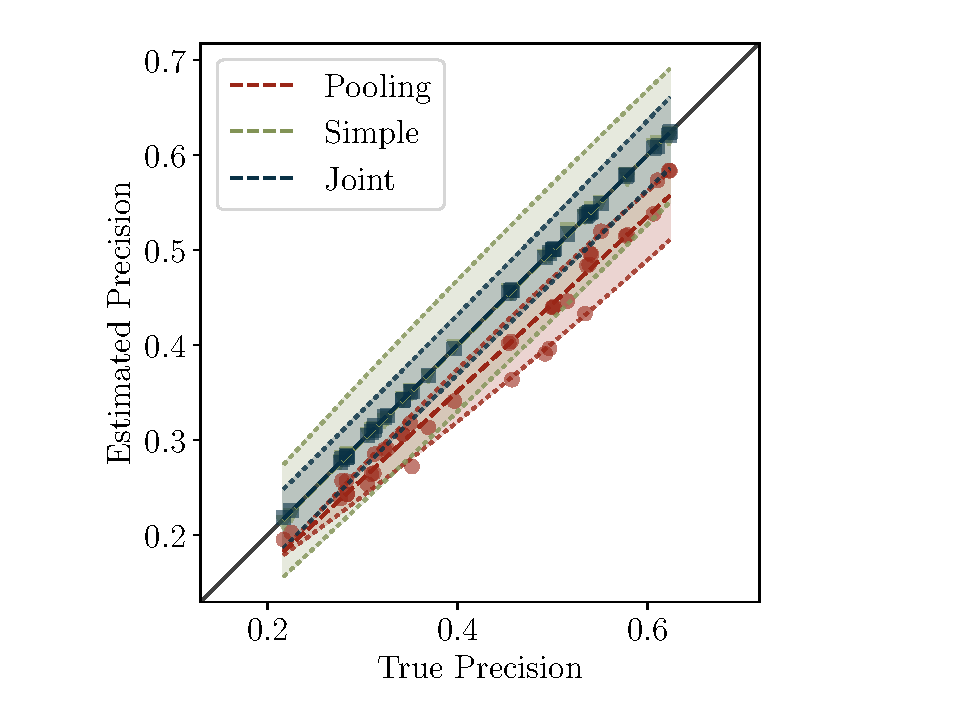
\includegraphics[width=\textwidth]{figures/simulation/simulation-p}
  \end{subfigure}
  \begin{subfigure}{0.49\textwidth}
    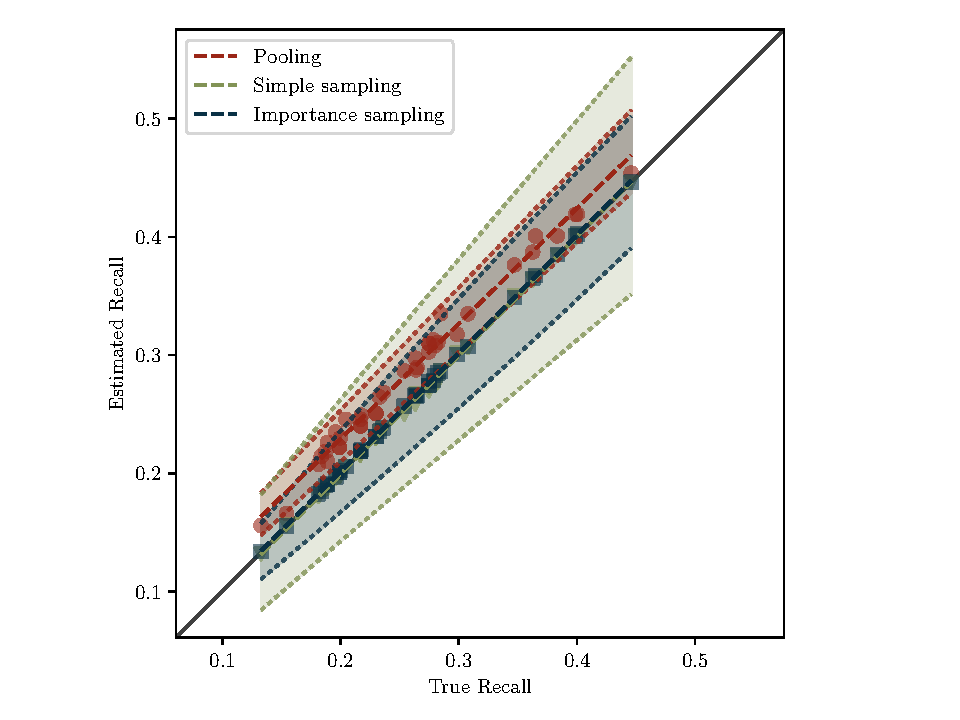
\includegraphics[width=\textwidth]{figures/simulation/simulation-r}
  \end{subfigure}
  \caption{\label{fig:simulation}
  A comparison of the pooling-based and sampling based estimators on a simulation of the TAC KBP 2015 challenge.
  While pooling-based estimates are biased, both the simple and importance-sampling based estimators in this work are unbiased.
  The importance-sampling estimate further has significantly reduced variance. 
  }
\end{figure*}

\subsection{Studying statistical properties with simulated experiments}
The statistical properties we'd like to study, namely bias and variance, require many repeated trials.
However, because the evaluation data in the TAC-KBP 2015 was collected by completely evaluating all predictions for 317 evaluation entities and 70 systems, we can simulate these trials by imagining that the evaluation data represents the universe of our output and treat a subset of the participating systems as submissions to our framework.

As baselines, we'll compare the precision and recall estimators proposed in \refsec{method} with the pooling-based methodology and with simple precision and recall estimators ($\pih^{(s)}$ and $\rhoh^{(s)}$) that do not reuse samples collected from other systems.
For the pooling-based methodology, we estimate bias and variance over many pool choices.
  On average, each pooled evaluation dataset has about \fake{1,000} evaluated instances.
For the sampling-based methodologies, we estimate bias and variance by running the experiment many times with about \fake{1,000} samples in total from all the different systems, making the two evaluation datasets comparable in terms of how many datapoints are drawn.

In \reffig{statistical-experiment}, we plot the precision and recall estimates made by each of these methods versus their ``true'' values which can be computed by looking at the entire evaluation corpus.
We see from the plots that the pooling-based methodology is significantly biased, while the sampling based estimators are not.
Furthermore, by incorporating samples drawn from other systems, the median variance reduces by a factor of \fake{4.1}, from \fake{0.2} (with the simple estimators) to \fake{0.05} (with the compound estimator).

\subsection{A mock evaluation for TAC-KBP 2016}
In \refsec{application}, we described the necessary elements required to apply on-demand open-world evaluation to KBP.
In particular, we needed to implement two crowd-worker interfaces to verify a relation tuple (i.e.\ evaluate $f(x)$) and to exhaustively annotate a document (i.e.\ to sample from $\sY$).
We have covered the cost and accuracy running these tasks in that section and will now study how well the evaluation framework works end to end. 

Using the algorithm described in \refalg{on-demand-sampling}, we evaluated three distinct relation extraction systems (a rule-based system, a supervised system and a neural network classifier) on 15,000 Newswire documents from 2016 TAC-KBP competition.
Each system uses Stanford CoreNLP~\citep{} to identify entities and the Illinois Wikifier~\citep{} to perform entity linking. 
In total, 100 documents were exhaustively annotated for about \$2,000, and 1000 of each systems submissions were annotated at about \$300 each, with 500 sampled to estimate macro-averaged relation scores and 500 were sampled to estimate macro-averaged entity scores.
\reffig{evaluation-results} presents the results of these systems on the mock evaluation.

\begin{figure}[t]
  \centering
  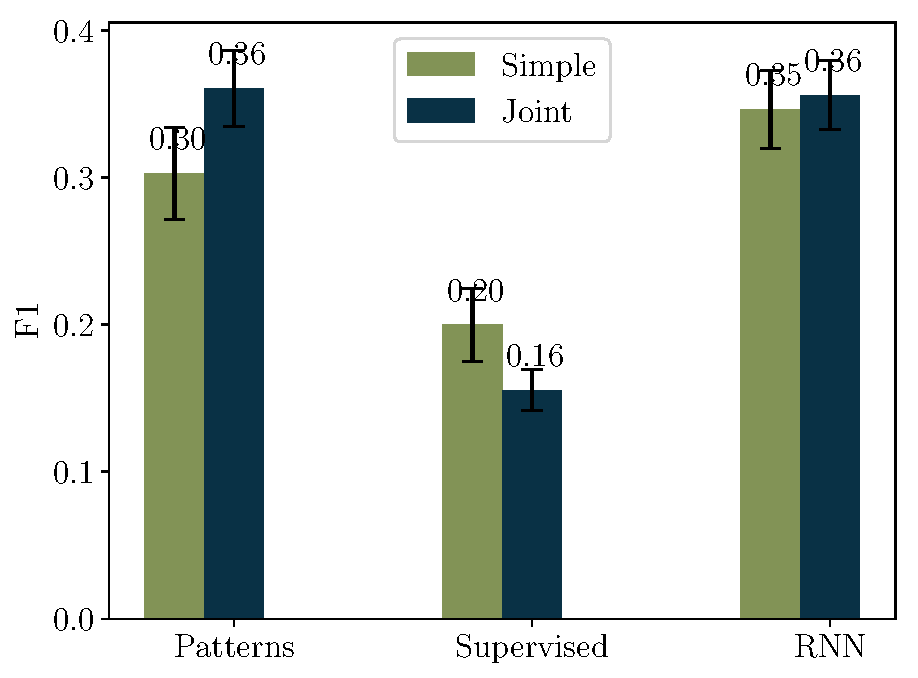
\includegraphics[width=\columnwidth]{figures/kbp2016/kbp2016_f1}
  \caption{\label{fig:evaluation-results} Results from a mock evaluation.}
\end{figure}

%\begin{table*}
%  \centering
%  \section{Evaluation}
\label{sec:evaluation}

Let us now see how well on-demand open-world evaluation works in practice.
We begin by empirically studying the statistical properties of the proposed estimators by simulating the evaluation procedure on the TAC-KBP 2015 evaluation data and show that the estimators are indeed unbiased and that pooling does reduce variance.
We then show that the on-demand open-world evaluation methodology can serve as a practical replacement for the TAC-KBP competitions by actually running a mock evaluation TAC-KBP 2016 competition using our framework and showing that we obtain results of comparable quality at a fraction of the cost.

\subsection{Studying statistical properties with simulated experiments}
The statistical properties we'd like to study, namely bias and variance, require many repeated trials.
However, because the evaluation data in the TAC-KBP 2015 was collected by completely evaluating all predictions for 317 evaluation entities and 70 systems, we can simulate these trials by imagining that the evaluation data represents the universe of our output and treat a subset of the participating systems as submissions to our framework.

As baselines, we'll compare the precision and recall estimators proposed in \refsec{method} with the pooling-based methodology and with simple precision and recall estimators ($\pih^{(s)}$ and $\rhoh^{(s)}$) that do not reuse samples collected from other systems.
For the pooling-based methodology, we estimate bias and variance over many pool choices.
  On average, each pooled evaluation dataset has about \fake{1,000} evaluated instances.
For the sampling-based methodologies, we estimate bias and variance by running the experiment many times with about \fake{1,000} samples in total from all the different systems, making the two evaluation datasets comparable in terms of how many datapoints are drawn.

In \reffig{statistical-experiment}, we plot the precision and recall estimates made by each of these methods versus their ``true'' values which can be computed by looking at the entire evaluation corpus.
We see from the plots that the pooling-based methodology is significantly biased, while the sampling based estimators are not.
Furthermore, by incorporating samples drawn from other systems, the median variance reduces by a factor of \fake{4.1}, from \fake{0.2} (with the simple estimators) to \fake{0.05} (with the compound estimator).

\subsection{A mock evaluation for TAC-KBP 2016}
In \refsec{application}, we described the necessary elements required to apply on-demand open-world evaluation to KBP.
In particular, we needed to implement two crowd-worker interfaces to verify a relation tuple (i.e.\ evaluate $f(x)$) and to exhaustively annotate a document (i.e.\ to sample from $\sY$).
We have covered the cost and accuracy running these tasks in that section and will now study how well the evaluation framework works end to end. 

Using the algorithm described in \refalg{on-demand-sampling}, we evaluated three distinct relation extraction systems (a rule-based system, a supervised system and a neural network classifier) on 15,000 Newswire documents from 2016 TAC-KBP competition.
Each system uses Stanford CoreNLP~\citep{} to identify entities and the Illinois Wikifier~\citep{} to perform entity linking. 
In total, 100 documents were exhaustively annotated for about \$2,000, and 1000 of each systems submissions were annotated at about \$300 each, with 500 sampled to estimate macro-averaged relation scores and 500 were sampled to estimate macro-averaged entity scores.
\tableref{evaluation-results} presents the results of these systems on the mock evaluation.

\begin{table*}
  \centering
  \begin{tabular}{l l c c c} \toprule
    Scheme      & System    & $P^e (\pm 95\%)$ & $R^e (\pm 95\%)$ & $\fone{}^e (\pm 95\%)$ \\ \midrule
\multirow{3}{*}{Uncombined} &
  Patterns   & \fake{80.4 $\pm$ 3.0}\% & \fake{10.4 $\pm$ 5.0}\% & \fake{18.41 $\pm$ 4.3}\% \\
& Supervised & \fake{60.4 $\pm$ 3.0}\% & \fake{15.4 $\pm$ 5.0}\% & \fake{24.54 $\pm$ 4.3}\% \\
& Neural     & \fake{20.4 $\pm$ 3.0}\% & \fake{30.4 $\pm$ 5.0}\% & \fake{24.41 $\pm$ 4.3}\% \\ \midrule
\multirow{3}{*}{+ Pooling} &
  Patterns   & \fake{80.4 $\pm$ 3.0}\% & \fake{10.4 $\pm$ 3.0}\% & \fake{18.41 $\pm$ 3.0}\% \\
& Supervised & \fake{60.4 $\pm$ 3.0}\% & \fake{15.4 $\pm$ 3.0}\% & \fake{24.54 $\pm$ 3.0}\% \\
& Neural     & \fake{20.4 $\pm$ 2.6}\% & \fake{30.4 $\pm$ 2.7}\% & \fake{24.41 $\pm$ 2.6}\% \\ \bottomrule
  \end{tabular}
  \caption{\label{tbl:evaluation-results} Results from a mock evaluation.}
\end{table*}

%\footnote{A summary of mention-level scores \fake{can be found in the appendix}.}  
% How does cost compare?
% How do absolute scores compare?
Two immediate takeaways are that the precisions of these systems are \fake{on par with} the precisions reported as part of the official 2016 evaluation but the 95\% confidence interval is \fake{almost three times smaller}.
The recall scores on this evaluation are a significantly smaller than on the official 2016 evaluation.
Our explanation for this is that the exhaustive annotation required by our system is far more expansive and finds a lot of new entities that our mention detection systems. \fake{More error analysis.}

%  \caption{\label{tbl:evaluation-results} Results from a mock evaluation.}
%\end{table*}

Two immediate takeaways are that the precisions of these systems are \fake{on par with} the precisions reported as part of the official 2016 evaluation but the 95\% confidence interval is \fake{almost three times smaller}.
The recall scores on this evaluation are a significantly smaller than on the official 2016 evaluation.
Our explanation for this is that the exhaustive annotation required by our system is far more expansive and finds a lot of new entities that our mention detection systems. \fake{More error analysis.}
